\documentclass{article}
\usepackage[final,main]{neurips_2026}
\usepackage[utf8]{inputenc}
\usepackage[T1]{fontenc}
\usepackage{hyperref}
\usepackage{url}
\usepackage{booktabs}
\usepackage{amsmath,amsfonts}
\usepackage{graphicx}
\usepackage{microtype}
\usepackage{xcolor}

\newcommand{\sha}[1]{\texttt{#1}}
\newcommand{\file}[1]{\texttt{\detokenize{#1}}}

\title{Vacuum-Flux Decomposition and a Grid Shape Model for Magnetics-Free Equilibrium Reconstruction}

\author{%
  Charlene Leong \\
  Independent \\
  \texttt{charleneleong84@gmail.com}
}

\begin{document}
\maketitle

\begin{abstract}
Methods report for the NeurIPS 2026 Fusion Equilibrium Challenge, status 11 October 2026 (development phase). We
reconstruct the DIII-D poloidal flux map $\psi(R,Z)$, $q_{95}$ and $\beta_N$ from coil currents and Thomson-scattering
profiles. $\psi$ is split into the analytic vacuum flux of the shipped coils and a learned plasma term, predicted by a
fixed-weight blend of 47 components: residual MLPs on PCA coefficients, XGBoost trees, a shape-target MLP ensemble and
three FiLM-conditioned U-Nets on the $65\times65$ grid. The best official DIII-D score is $S = 0.993927$ (rank 29 of
50), up from 0.990496 for the first entry; the leaders are at 0.9964--0.9967. Every blend weight since 8 October was
chosen on 160 never-scored held-out shots. MAST (Challenge 2) is zero-shot and label-free: $S_{\mathrm{MAST}} =
0.627752$, $G = 0.631588$. We report the full funnel, the closed directions, and what is not established.
\end{abstract}

\section{Task}
\label{sec:task}
Each tokamak shot gives coil currents, plasma current $I_p$ and Thomson $T_e$/$n_e$ profiles; the targets are the
EFIT flux map on a $65\times65$ grid and $q_{95}$, $\beta_N$ at every EFIT time. Challenge~1 scores DIII-D with
\[
S = 0.55\,R^2_\psi + 0.15\,R^2_{q_{95},\beta_N} + 0.10\,(1 - D_{\mathrm{LCFS}}) + 0.20\,\mathrm{Consistency},
\]
where Consistency is the mean $R^2$ of seven scalars the scorer derives from the predicted flux ($R_{\mathrm{axis}}$,
$Z_{\mathrm{axis}}$, $\kappa$, upper and lower triangularity, volume, $l_i$). Challenge~2 scores zero-shot transfer to
MAST as $G = S_{\mathrm{MAST}} / S_{\mathrm{DIII\text{-}D}}$. The data are 7{,}041 \file{diii_d_train} shots, 874
\file{diii_d_public_test} shots and 1{,}206 \file{mast_public_test} shots; there is no MAST training set, and the three
labelled MAST demo shots are for inspection only (rule~3). The development phase closes 18 October; the Final phase
(19--26 October, 3 submissions) requires a reproduction package that trains within 24 A100-hours.

\section{Method}
\label{sec:method}
\paragraph{Inputs and vacuum flux.} Coil currents and $I_p$ are interpolated onto the EFIT times (with the organisers'
$I_p$ time-axis errata applied), and Thomson profiles are resampled onto fixed spatial stations so shots with different
channel layouts share one feature space. The vacuum flux $\psi_{\mathrm{vac}}(R,Z) = \sum_c I_c G_c(R,Z)$ uses
circular-filament elliptic-integral Green's functions over each shipped coil rectangle; it is exact, linear, and
defined on any machine from its geometry alone (\file{fusioneq/greens.py}).

\paragraph{Base ensemble (flux level).} Residual MLPs (2048 wide, depth 10, 120 epochs, bf16, a 50/50 mix of the
coefficient and pixel losses) predict PCA coefficients of the plasma flux plus $q_{95}$ and $\beta_N$. Fifteen members
are averaged (v5, v6 and v8 seeds and region-loss runs, and six ramp-weighted v14 members), and XGBoost on the host
network's inputs for the top 32 PCA coefficients is blended in at 0.1. The submitted $q_{95}$ and $\beta_N$ come from
this ensemble.

\paragraph{Shape-target hybrid.} 27 MLPs (v16--v21) predict the flux \emph{shape}: $\psi$ centred and scaled by its
own mean and spread inside the scorer's envelope. Their average is moved onto the base flux's envelope mean and spread
(\file{match_envelope}), so it contributes shape (consistency, boundary) without its weaker level. XGBoost trees on the
top 32 shape-PCA coefficients (host \file{v21_normalize_seeds_i00}) add a second shape family.

\paragraph{Grid shape model.} A U-Net on the grid padded to $72\times72$ (three downsamplings) maps the vacuum flux in
shape units and the $R$, $Z$ coordinate maps to the flux shape; the frame's feature vector (coil currents, $I_p$,
Thomson with $\pm4$ frames of context) enters through an MLP that scales and shifts every level's channels (FiLM). The
loss is pixel MSE in shape units, weighted up inside the envelope; training uses AdamW with a one-cycle schedule and
bf16 autocast, keeping the epoch with the lowest validation envelope loss (\file{fusioneq/grid.py},
\file{docs/specs/2026-10-08-grid-shape-model-design.md}). Table~\ref{tab:grid} lists the trained variants.

\begin{table}[h]
\centering
\caption{Grid models. Envelope loss is on the 40 never-scored validation shots.}
\label{tab:grid}
\small
\begin{tabular}{llcc}
\toprule
Model & Data & Channels / epochs & Validation envelope loss \\
\midrule
grid\_v1 & every 2nd frame & 32 / 10 & 0.00105 \\
grid\_v2 & all frames & 48 / 15 & 0.00075 \\
grid\_v2\_s1 & all frames, seed 1 & 48 / 15 & 0.00065 \\
grid\_v3 & all frames & 64 / 20 & 0.00064 \\
grid\_v2\_gs & all frames, Grad-Shafranov loss weight 50 & 48 / 15 & 0.0031 (closed) \\
\bottomrule
\end{tabular}
\end{table}

\paragraph{Blend.} The submitted flux is
$\psi = w_b\,\mathrm{base} + w_h\,\mathrm{hybrid} + w_{st}\,\mathrm{shape\ trees} + w_g\,\overline{\mathrm{grid}}$,
with each shape component moved onto the base's envelope statistics (\file{fusioneq/blend.py}). The official best
(\file{configs/blends/v21_27_grids3.yaml}) uses $w_b = 0.10$, $w_h = 0.10$, $w_{st} = 0.15$, $w_g = 0.65$ over
grid\_v2, grid\_v2\_s1 and grid\_v3. MAST uses no learned model (Section~\ref{sec:mast}).

\section{Evaluation protocol}
\label{sec:protocol}
A fixed shot-level split (seed 0) holds out 200 training shots. The first 40 are the \emph{scoring} shots that every
local number in the sweep writeups is reported on; the other 160 (40 \emph{validation} plus 120 \emph{spare}) are never
used for those scores. From 8 October, every blend weight is screened on five 40-shot groups (spare thirds 1--3,
validation, scoring) as paired deltas against the current official best, and pooled over the 160 never-scored shots
(\file{docs/experiments/fusioneq/screens.yaml}). Two promotion gates
(\file{docs/experiments/fusioneq/verdicts.yaml}):
\begin{itemize}
\item \textbf{G1}: beats the matched-seed baseline on the 40 scoring shots by more than seed noise (0.0013 for one
  model, about 0.0002 for an ensemble).
\item \textbf{G2}: lifts the blend on held-out shots (from 8 October: wins most 40-shot groups of the 160 never-scored
  shots), then beats the official best on Codabench.
\end{itemize}
\textbf{Both gates were tightened after seeing results.} The seed-noise threshold in G1 was measured in v6 (seeds 1
and 2 of the v5 winner scored 0.9901--0.9902 against 0.9915), after v5 had been promoted on what turned out to be a
lucky seed. The 160-shot group rule in G2 was added on 8 October after two local gains failed to transfer: temporal
smoothing (+0.00018 on the scoring shots; 0.992144 officially against 0.992168) and v21's six extra members (+0.00007
locally, $-0.000004$ officially). Neither gate was pre-registered for the experiments that motivated it. The MAST
solenoid-shape correction (\sha{4c428222}) was chosen by official feedback, not by a local gate.

\section{Results on DIII-D}
\label{sec:results}

\begin{table}[h]
\centering
\caption{Official DIII-D submissions that set a new best (\file{results/codabench.json}). $D$ is
$D_{\mathrm{LCFS}}$; rank is on the Codabench public test where recorded.}
\label{tab:official}
\footnotesize
\setlength{\tabcolsep}{4pt}
\begin{tabular}{llccccl}
\toprule
Date & HF commit & $S$ & $R^2_\psi$ & $D$ & Cons. & What changed \\
\midrule
29 Sep & \sha{15903ed1} & 0.990496 & 0.999586 & 0.013063 & 0.963719 & one residual MLP (v5), rank 30 \\
29 Sep & \sha{d992d040} & 0.991639 & 0.999730 & 0.012340 & 0.968326 & 3-seed ensemble, rank 29 \\
30 Sep & \sha{07a1ba61} & 0.992005 & 0.999758 & 0.012114 & 0.969830 & 5-model ensemble, rank 28 \\
30 Sep & \sha{df98320e} & 0.992168 & 0.999765 & 0.012034 & 0.970494 & 9-model ensemble (v8), rank 26 of 77 \\
3 Oct & \sha{ccb9ef31} & 0.992317 & 0.999762 & 0.012058 & 0.971258 & + 0.1 XGBoost coefficient trees \\
4 Oct & \sha{f4205360} & 0.992341 & 0.999753 & 0.012031 & 0.971439 & + six ramp-weighted members \\
5 Oct & \sha{9e381a13} & 0.992663 & 0.999759 & 0.011780 & 0.972906 & + shape-target hybrid (3 members) \\
6 Oct & \sha{5cae79d2} & 0.992830 & 0.999760 & 0.011645 & 0.973671 & 6 shape members at 0.5 \\
6 Oct & \sha{0c9a8ac9} & 0.992904 & 0.999760 & 0.011559 & 0.973998 & 12 shape members at 0.65 \\
7 Oct & \sha{7a56d52a} & 0.993078 & 0.999762 & 0.011437 & 0.974805 & 21 members + shape trees, rank 28 \\
8 Oct & \sha{12068a0d} & 0.993114 & 0.999764 & 0.011437 & 0.974978 & trees on 2x data, rank 28 \\
9 Oct & \sha{93605aab} & 0.993186 & 0.999767 & 0.011510 & 0.975366 & + grid\_v1 at 0.1, rank 29 \\
9 Oct & \sha{d3076dea} & 0.993520 & 0.999773 & 0.011495 & 0.977012 & grid\_v2 at 0.5, rank 28 \\
10 Oct & \sha{9c2c5fab} & 0.993769 & 0.999776 & 0.011233 & 0.978119 & two grid seeds at 0.6, rank 28 \\
11 Oct & \sha{07cfd3ff} & \textbf{0.993927} & 0.999777 & 0.011025 & 0.978802 & three grids at 0.65, rank 29 of 50 \\
\bottomrule
\end{tabular}
\end{table}

\begin{figure}[h]
  \centering
  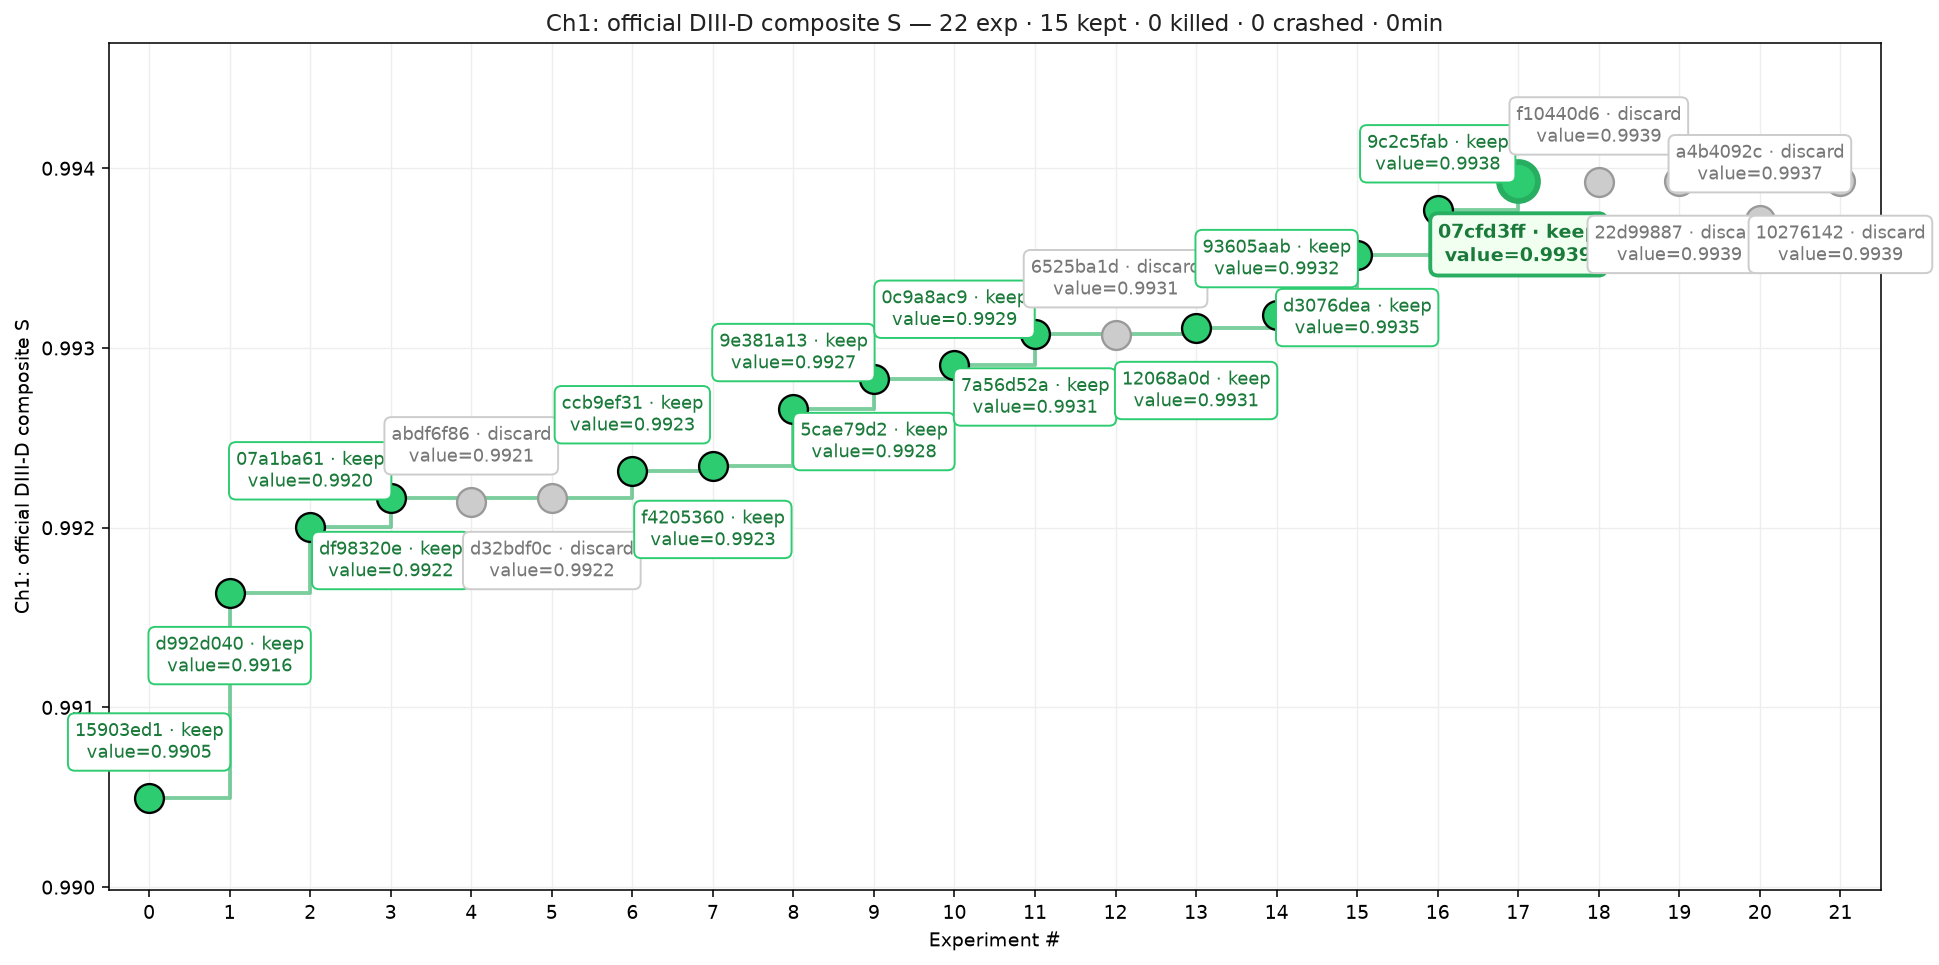
\includegraphics[width=\linewidth]{../experiments/progress/official/ch1_diii_d.png}
  \caption{Official DIII-D $S$ per scored DIII-D prediction file, with the running best. Grey points did not beat the
  best: temporal smoothing (\sha{abdf6f86}), a MAST-only change resubmitting the \sha{df98320e} DIII-D file
  (\sha{d32bdf0c}), and the 27-member blend (\sha{6525ba1d}).}
  \label{fig:progress}
\end{figure}

Two model families account for most of the second half. The shape target lifted the official score by +0.00049 in two
submissions (\sha{f4205360} to \sha{5cae79d2}); the grid model by +0.00081 in four (\sha{12068a0d} to
\sha{07cfd3ff}), mostly through consistency (0.974978 $\to$ 0.978802). Adding members to an existing family stopped
paying after the 9-model ensemble (13 and 17 members: 0.99277 and 0.99272 locally against 0.99277), and
$R^2_{q_{95},\beta_N}$ has been 0.995946 in every submission since 4 October. In the 160-shot screens
(Table~\ref{tab:screens}) each of the four grid submissions was positive in all five 40-shot groups.

\begin{table}[h]
\centering
\caption{Screens of the grid blends: paired $\Delta S \times 10^{-6}$ per 40-shot group against the previous official
best, and pooled $S$ on the 160 never-scored shots (\file{docs/experiments/fusioneq/screens.yaml}). The w75 candidate
has not been submitted.}
\label{tab:screens}
\small
\begin{tabular}{lccccccc}
\toprule
Blend & spare 1 & spare 2 & spare 3 & valid. & scoring & $S_{160}$ & Official \\
\midrule
grid\_v1 at 0.1 & 87 & 83 & 191 & 63 & 73 & -- & 0.993186 \\
grid\_v2 at 0.5 & 441 & 502 & 2166 & 445 & 301 & 0.993167 & 0.993520 \\
two grids at 0.6 & 288 & 340 & 1101 & 207 & 54 & 0.993643 & 0.993769 \\
three grids at 0.65 & 171 & 150 & 557 & 200 & 102 & 0.993914 & 0.993927 \\
grids at 0.75 (w75) & 21 & 15 & 190 & 130 & 39 & 0.994000 & not scored \\
\bottomrule
\end{tabular}
\end{table}

On the 40 local scoring shots the official best blend scores $S = 0.994341$ (validation shots 0.993694) against
0.993927 officially; the local scoring shots have run high since the first entry (0.9915 locally against 0.9905
officially). Against the leaders (0.9964--0.9967) the gap is mostly consistency (0.9788 against about 0.988, weakest
in $\kappa$ and $l_i$), then the boundary ($D_{\mathrm{LCFS}}$ 0.0110 against 0.007) and $q_{95}$/$\beta_N$ (0.9959
against 0.998; \file{docs/journey.md}). Projecting the true flux onto the base model's 192-component PCA scores
0.9988, so the representation is not the limit (\file{docs/diii-d-diagnosis.md}).

\section{The funnel}
\label{sec:funnel}
Table~\ref{tab:funnel} counts every stage, including runs that were killed or never scored.

\begin{table}[h]
\centering
\caption{From trained runs to the submitted blend. Sources: \file{configs/schedules/}, the sweep writeups in
\file{docs/experiments/fusioneq/mlp/}, \file{verdicts.yaml}, \file{screens.yaml}, \file{results/codabench.json}, and
the git log of 11 October.}
\label{tab:funnel}
\small
\begin{tabular}{p{0.23\linewidth}p{0.70\linewidth}}
\toprule
Stage & Count \\
\midrule
MLP sweeps (v1--v21) & 21 schedules, 115 scheduled iterations (trainings plus ensemble iterations). Not completed as
scheduled: 3 of v2's (cut after 2 of 5), 2 of v4's (killed by a false-positive memory triage), 4 of v15's (killed by
the GPU-hang triage, rerun as v15b). \\
Grid models & 6 started: grid\_v1, grid\_v2, grid\_v2\_s1, grid\_v3, grid\_v2\_gs, and grid\_v4 (96 channels), which
was lost to an OOM kill on 11 October and is retraining. grid\_v3\_ctx8 and grid\_v3\_env8 are being re-run. \\
Experiments with a verdict & 27: 11 PROMOTE, 5 KEEP, 11 DISCARD. \\
Blend screens & 12 candidates in \file{screens.yaml}, 6 of them submitted. On 11 October two blend builds were
OOM-killed on the shared host (before \file{blend --no-score}), and every w75 build was OOM-killed (count not recorded)
before the compact XGBoost loader. \\
Official submissions & 35 rows in \file{codabench.json}: 3 candidates held back, 1 submitted without a separate score,
31 scored. They carry 17 distinct DIII-D prediction files; 15 set a new best (Table~\ref{tab:official}) and 2 did
not. \\
Submitted blend & 47 components: 15 base MLPs, 1 coefficient-tree model, 27 shape-target MLPs, 1 shape-tree model and
3 grid models. \\
\bottomrule
\end{tabular}
\end{table}

\section{Cross-machine transfer (MAST)}
\label{sec:mast}
The learned models ingest DIII-D coils, so MAST gets a physics flux: its coil vacuum flux plus the measured plasma
current spread as $J \propto (1-\rho^2)^\alpha$ over an ellipse placed where the Thomson density exceeds a fraction of
its peak (\file{fusioneq/plasma.py}, \file{fusioneq/physics.py}). A global scale ($-0.8724$), a plasma-to-vacuum ratio
($0.9005$) and an offset ($-0.0201$) are fitted on DIII-D training shots, where labels are allowed
(\file{results/mast_physics.json}); the current entry uses $\alpha = 2.0$ and a threshold fraction of 0.4. $q_{95}$ and
$\beta_N$ come from textbook formulas on the predicted boundary, the toroidal field and the Thomson pressure
(volume-averaged $\beta_N$).

\begin{table}[h]
\centering
\caption{Official MAST rows (\file{results/codabench.json}). $R^2_\psi$ is after the scorer's global sign flip.
\sha{f4fa3fea} used terms fitted on the three labelled demo shots, which rule~3 forbids in the Final phase.}
\label{tab:mast}
\footnotesize
\setlength{\tabcolsep}{4pt}
\begin{tabular}{llcccccc}
\toprule
HF commit & MAST flux & $S_{\mathrm{MAST}}$ & $R^2_\psi$ & $R^2_{q,\beta}$ & $D$ & Cons. & $G$ \\
\midrule
\sha{15903ed1} & vacuum only & 0 & -- & -- & -- & -- & 0 \\
\sha{737ce338} & calibrated physics flux & 0.557707 & 0.873347 & $-0.259401$ & 0.244564 & 0.009112 & 0.563058 \\
\sha{d32bdf0c} & $\alpha$ 2.0, frac 0.4, vol.\ $\beta_N$ & 0.604496 & 0.877339 & 0.320132 & 0.260607 & 0 & 0.609268 \\
\sha{f4fa3fea} & + demo-fitted offset, lines & 0.644578 & 0.935922 & 0.372570 & 0.260645 & 0 & 0.649666 \\
\sha{f2b36e3e} & label-free, half solenoid & 0.540680 & 0.749632 & 0.320132 & 0.219799 & 0.011712 & 0.544070 \\
\sha{4c428222} & label-free, solenoid shape & \textbf{0.627752} & 0.907922 & 0.320132 & 0.219674 & 0.011711 &
0.631688 \\
\bottomrule
\end{tabular}
\end{table}

The current entry is label-free: \sha{4c428222} adds the shape part of halving the solenoid current (each frame's
correction minus its grid mean, so the level is kept), which recovers about 58\% of the banned offset's gain. With the
\sha{07cfd3ff} DIII-D file it gives $G = 0.631588$. The remaining $R^2_\psi$ error is mostly a per-frame level: on the
demo shots one global offset lifts $R^2_\psi$ from 0.827 to 0.892 and the right per-frame offset to 0.957, and that
offset tracks the solenoid current (correlation $-0.99$). A coil-geometry audit against published MAST geometry found
no geometry error, so vessel currents are the suspect; nothing label-free calibrates them
(\file{docs/mast-diagnosis.md}).

\paragraph{Disclosure: how $\alpha$ and the Thomson threshold were chosen.} $\alpha = 2.0$ and the 0.4 threshold
fraction were shortlisted by a 36-setting sweep scored on the three labelled MAST demo shots (demo $S$ 0.537 $\to$
0.584), which rule~3 now restricts to format inspection. No parameter is fitted to the demo shots and no demo-derived
term enters the prediction. We keep the two values because official Development feedback, which rule~3 permits for
comparing and selecting MAST pipelines, backs them: \sha{d32bdf0c} ($\alpha = 2.0$, 0.4) scored MAST $S$ 0.604496
against 0.6017 for \sha{501b7986} (the previous setting), raising $R^2_\psi$ 0.873 $\to$ 0.877 and $R^2_{q_{95},\beta_N}$
0.294 $\to$ 0.320 while consistency fell 0.009 $\to$ 0 and $D_{\mathrm{LCFS}}$ rose 0.245 $\to$ 0.261. The $q_{95}$
aspect-ratio cap of 0.65 was likewise compared officially against 0.7 (0.6017 against 0.6004). The organisers may read
rule~3 more strictly; the label-free alternative is to re-select both values on official feedback alone.

\section{Closed directions}
\label{sec:closed}
\begin{table}[h]
\centering
\caption{Do not retry (\file{verdicts.yaml}, \file{docs/mast-diagnosis.md}, \file{docs/journey.md}).}
\label{tab:closed}
\small
\begin{tabular}{p{0.23\linewidth}p{0.70\linewidth}}
\toprule
Direction & Measured result and reason \\
\midrule
Grad-Shafranov loss on the grid model & At weight 50 the validation envelope loss rises to 0.0031 (grid\_v2: 0.00075).
On 160 shots it loses to the \sha{07cfd3ff} blend (0.993914) as an extra grid (0.993827), as a replacement (0.993863)
and alone (0.992890). Closed unless retried at weight 5 or less. \\
Free-boundary Grad-Shafranov for MAST shape & Checked on DIII-D, where labels are allowed: pinned centroid $S$ 0.5035,
consistency 0, $R^2$ of $R_{\mathrm{axis}}$ $-9.2$ and of $\kappa$ $-11.4$; free centroid $S$ 0.392. Without
magnetics or vessel currents nothing holds the plasma shape. \\
Demo-fitted offsets on MAST & A solenoid offset and $q_{95}$/$\beta_N$ lines fitted on the 3 labelled demo shots took
MAST to 0.644578, but rule~3 forbids demo-shot fits in Final submissions. \\
Machine-agnostic grid model & Stopped at gate 0: DIII-D's plasma cannot be placed from Thomson the MAST way ($R_0$
correlation $-0.16$, $a$ correlation 0.19 with EFIT), so the model could only learn a typical DIII-D plasma. A learned
MAST flux correction had already lowered MAST $S$ from 0.575 to 0.521. \\
More of one family & 13 and 17 MLP members, wider (4096) or longer (240-epoch) members, the 160 spare shots as
training data, whole-shot temporal models, full-resolution Thomson, history features: all flat or negative under G1. \\
\bottomrule
\end{tabular}
\end{table}

\section{What is not established}
\label{sec:not-established}
\begin{itemize}
\item \textbf{The w75 re-weighting.} Grids at 0.75 score 0.994000 on the 160 never-scored shots (+0.000086 over
  \sha{07cfd3ff}, positive in all five groups), but it has not been scored officially, and the gain is below the size
  of past 160-to-official gaps.
\item \textbf{Running grid variants.} grid\_v3\_ctx8 ($\pm8$ frames of context) and grid\_v3\_env8 (heavier envelope
  weight) are being re-run, and grid\_v4 (96 channels) is retraining after an OOM kill; none has a 160-shot result.
\item \textbf{Group-level evidence is coarse.} Shot-level discordant counts are not recorded; with five paired 40-shot
  deltas a sign test reaches $p = 0.031$ at best.
\item \textbf{MAST $R^2_\psi = 0.908$.} The per-frame level error that scales with the solenoid current is
  unexplained; vessel currents are the suspect and are untested. Our MAST consistency is 0.0117, while higher-ranked
  teams reach 0.24--0.89, and we do not know how. The demo-shot shortlist for $\alpha$ and the Thomson
  threshold is disclosed in Section~\ref{sec:mast}; whether the organisers accept official feedback as the deciding
  evidence is theirs to rule.
\item \textbf{The consistency gap.} 0.9788 against about 0.988 for the leaders, weakest in $\kappa$ and $l_i$; its
  cause is not identified.
\item \textbf{$q_{95}$ / $\beta_N$.} Fixed at 0.995946 since 4 October. Direct heads and XGBoost on the scalars did not
  beat the base ensemble (+0.000055 validation, $-0.000033$ scoring), and how the leaders reach 0.998 is not known.
\item \textbf{Final-phase reproduction.} Retraining the 47-component blend from the pinned commit within 24 A100-hours,
  and rebuilding the label-free MAST entry end to end, is untested. Per-member training times are logged in the sweep
  writeups (18--46\,min for shape-target members), but the blend's total compute has not been summed.
\end{itemize}

\section{Reproducibility}
\label{sec:repro}
Code: \file{competitions/fusion-equilibrium/}, entry points in \file{fusioneq.cli} (\file{prepare}, \file{train},
\file{train-grid}, \file{blend}, \file{build}). Blend specs: \file{configs/blends/*.yaml}; sweep recipes:
\file{configs/schedules/}. Locked versions (\file{uv.lock}): torch 2.14.0, xgboost 3.2.0, numpy 1.26.4, scikit-learn
1.9.1, autoresearch 0.38.0. Predictions are pushed to the private HF dataset \file{chaleong/fusion-eq-predictions}; the
official best is HF commit \sha{07cfd3fffbf78a0b012f384291e269d9b4318698}. Experiment card:
\file{docs/experiment-card.md}. W\&B project: \file{chaleong/fusion-equilibrium}.

\end{document}
